\documentclass[aspectratio=169, 14pt]{beamer}
\usepackage{beamerthemeTalentSprint}
\usepackage{tcolorbox}
\usepackage{booktabs}
\usepackage{amsmath}
\usepackage{tikz}
\usepackage{csquotes}
\usetikzlibrary{shapes, shadows, arrows}
\tikzstyle{arrow} = [thick, ->, >=stealth, color =black,line width = 1.5pt]
\tikzstyle{circle} = [circle,draw=blue!50,fill=blue!20,thick]
\tikzstyle{block} = [rectangle, draw=black, thick,text width=1.2cm, text centered, font=\tiny]
\title[Support Vector Machines]{Support Vector Machines}



\begin{document}

{\1
\begin{frame}
	\title{Non - Linear SVM}​
\titlepage
\end{frame}
}


\begin{frame}[t]{Introduction to SVM: Why SVIM?}
\begin{itemize}
\itemsep1em 
\item<2->  Working with neural networks for supervised and unsupervised learning showed good results while used for such learning applications.
\item<3->  MLP's uses feed forward and recurrent networks.
\item<4->  Multilayer perceptron (MLP) properties include universal approximation of continuous nonlinear functions and include learning with input-output patterns and also involve advanced network architectures with multiple inputs and outputs.

\end{itemize}
\end{frame}


\begin{frame}[t]{Introduction to SVM: Why SVIM?}
\begin{itemize}
\itemsep1em 
\item<2->  There can be some issues noticed. Some of them are having many local minima and also finding how many neurons might be needed for a task is another issue which determines whether optimality of that NN is reached.
\item<3->  Another thing to note is that even if the neural network solutions used tends to converge, this may not result in a unique solution.
\end{itemize}
\end{frame}

\begin{frame}[t]{Introduction to SVM: Why SVIM?}
\begin{columns}
	\begin{column}{0.55\textwidth}
        \begin{itemize}
          \itemsep1em 
	  \item Now let us look at another example where we plot the data and try to classify it and we see that there are many hyper planes which can classify it.
         \item But which one is better?
	\end{itemize}
	\end{column}
	\begin{column}{0.45\textwidth}
		\vskip-0.5cm
		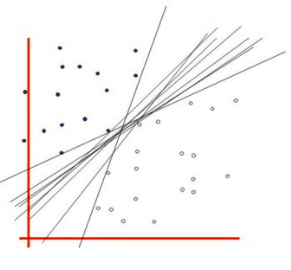
\includegraphics[width=0.9\textwidth]{SVM_NonLinear_Images/AIML_SVM_IMG1.png}
		\end{column}
\end{columns}

\end{frame}



\begin{frame}[t]{Linear classifier}
\begin{columns}
	\begin{column}{0.55\textwidth}
	\begin{itemize}
	  \item Decision boundary: Hyperplane
	\end{itemize}
	\[ w^{T} x=0 \]

	\begin{itemize}
	  \item Class 1 lies on the positive side
	\end{itemize}
	\[ w^{T} x>0 \]


	\begin{itemize}
	  \item Class 0 lies on the negative side
	\end{itemize}
        \[ w^{T} x<0 \]

	\end{column}
	\begin{column}{0.45\textwidth}
		\vskip-0.5cm
                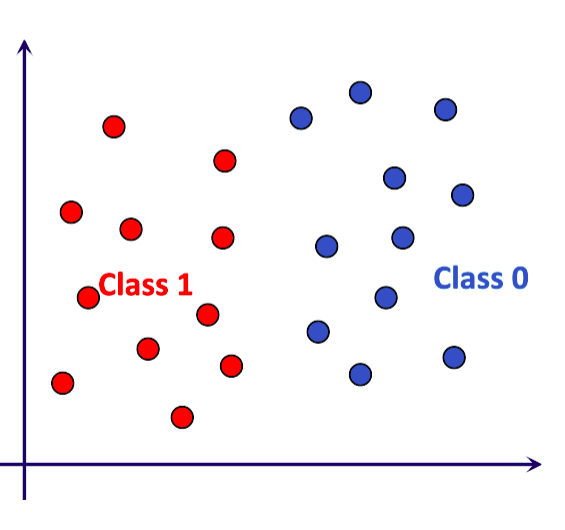
\includegraphics[width=0.9\textwidth]{SVM_NonLinear_Images/AIML_SVM_IMG2.png}
	\end{column}
\end{columns}

\end{frame}

\begin{frame}[t]{Linear classifier}
\begin{columns}
	\begin{column}{0.55\textwidth}
	\begin{itemize}
	  \item Decision boundary: Hyperplane
	\end{itemize}
	\[ w^{T} x=0 \]

	\begin{itemize}
	  \item Class 1 lies on the positive side
	\end{itemize}
	\[ w^{T} x>0 \]


	\begin{itemize}
	  \item Class 0 lies on the negative side
	\end{itemize}
        \[ w^{T} x<0 \]

	\end{column}
	\begin{column}{0.45\textwidth}
		\vskip-0.5cm
                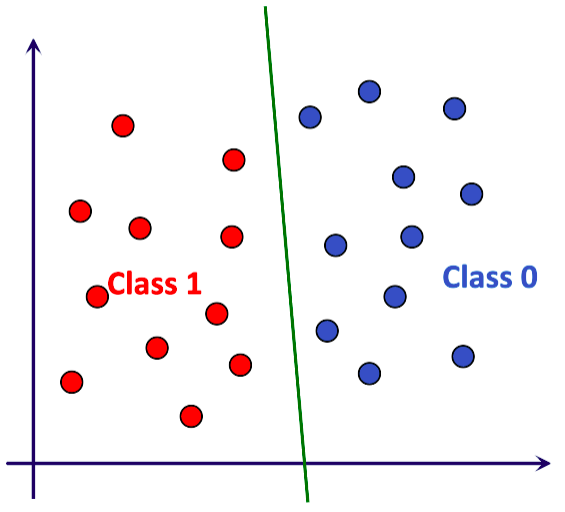
\includegraphics[width=0.9\textwidth]{SVM_NonLinear_Images/AIML_SVM_IMG3.png}
	\end{column}
\end{columns}

\end{frame}

\begin{frame}[t]{Linear classifier}
\begin{columns}
	\begin{column}{0.55\textwidth}
	\begin{itemize}
	  \item Decision boundary: Hyperplane
	\end{itemize}
	\[ w^{T} x=0 \]

	\begin{itemize}
	  \item Class 1 lies on the positive side
	\end{itemize}
	\[ w^{T} x>0 \]


	\begin{itemize}
	  \item Class 0 lies on the negative side
	\end{itemize}
        \[ w^{T} x<0 \]

	\end{column}
	\begin{column}{0.45\textwidth}
		\vskip-0.5cm
		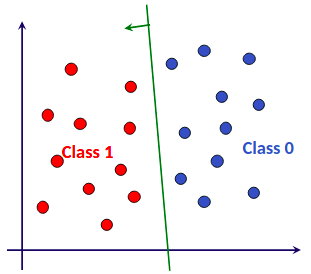
\includegraphics[width=0.9\textwidth]{SVM_NonLinear_Images/AIML_SVM_IMG4.png}
	\end{column}
\end{columns}

\end{frame}


\begin{frame}[t]{Summary: Max-Margin Classification​}
\begin{columns}
	\begin{column}{0.55\textwidth}
        \begin{itemize}
	\item A Large Margin will reduce the chance of misclassifying future test samples
	\item In other words, large-margin classifiers will generalize better.​
        \item Samples at the boundary support the margin: called Support Vectors
	\end{itemize}
	\end{column}
	\begin{column}{0.45\textwidth}
		\vskip-0.5cm
		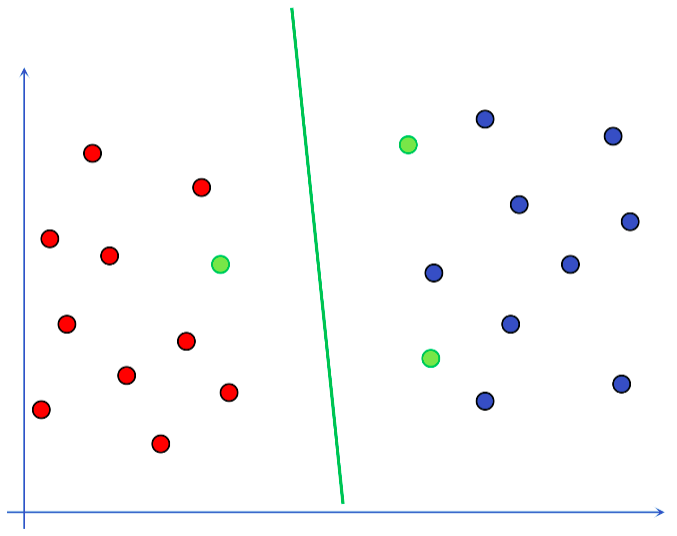
\includegraphics[width=0.9\textwidth]{SVM_NonLinear_Images/AIML_SVM_IMG5.png}
        \end{column}
\end{columns}

\end{frame}


\begin{frame}[t]{Summary: Max-Margin Classification​}
\begin{columns}
	\begin{column}{0.55\textwidth}
        \begin{itemize}
	\item A Large Margin will reduce the chance of misclassifying future test samples
	\item In other words, large-margin classifiers will generalize better.​
        \item Samples at the boundary support the margin: called Support Vectors
	\end{itemize}
	\end{column}
	\begin{column}{0.45\textwidth}
		\vskip-0.5cm
		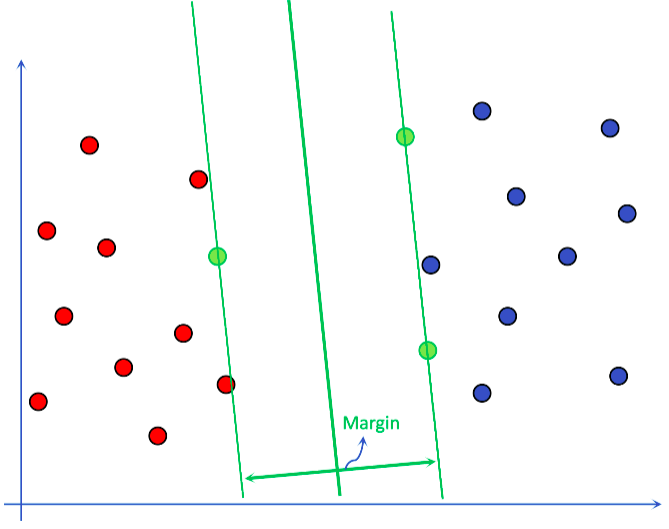
\includegraphics[width=0.9\textwidth]{SVM_NonLinear_Images/AIML_SVM_IMG6.png}
        \end{column}
\end{columns}

\end{frame}

\begin{frame}[t]{Summary: Max-Margin Classification​}
\begin{columns}
	\begin{column}{0.55\textwidth}
        \begin{itemize}
	\item A Large Margin will reduce the chance of misclassifying future test samples
	\item In other words, large-margin classifiers will generalize better.​
        \item Samples at the boundary support the margin: called Support Vectors
	\end{itemize}
	\end{column}
	\begin{column}{0.45\textwidth}
		\vskip-0.5cm
		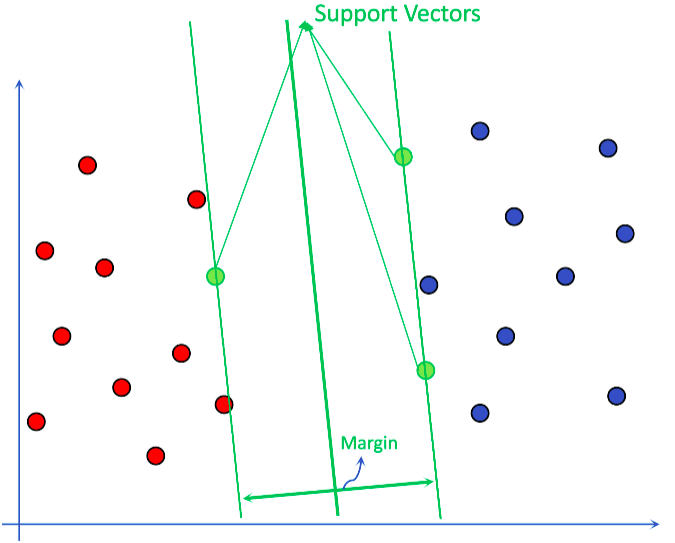
\includegraphics[width=0.9\textwidth]{SVM_NonLinear_Images/AIML_SVM_IMG7.png}
        \end{column}
\end{columns}

\end{frame}


\begin{frame}[t]{Non Linear SVM}
\begin{itemize}
  \item Some data points are not linear separable
  \item \textbf{Intuition}: to transform the data to a high dimension space
\end{itemize}
\center
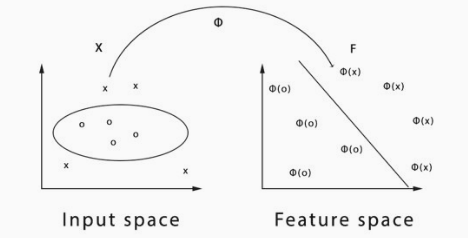
\includegraphics[width=0.6\textwidth]{SVM_NonLinear_Images/AIML_SVM_IMG8.png}
\end{frame}

\begin{frame}[t]{Support Vector Machines}
\begin{columns}
	\begin{column}{0.55\textwidth}
        \begin{itemize}
	\item SVM uses kernel to transform the data and then based on these transformations it finds an optimal hyperplane that distinctly classifies the data points.
	\item Example:\\
	  -No Straight line that can separate the two groups
	\end{itemize}
	\end{column}
	\begin{column}{0.45\textwidth}
		\vskip-0.5cm
		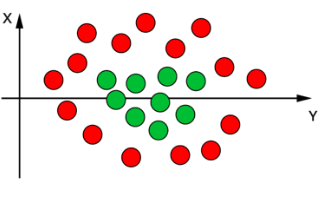
\includegraphics[width=0.9\textwidth]{SVM_NonLinear_Images/AIML_SVM_IMG9.png}
        \end{column}
\end{columns}
\end{frame}



\begin{frame}[t]{Transform}
\begin{columns}
	\begin{column}{0.55\textwidth}
        \begin{itemize}
	\item Transform the data by adding one more dimension as z\
              - where z = $x^{2} + y^{2}$
	\item If we plot in z-y axis, a clear speration is visible  and a line can drawn
        \item The line is the hyperplane we want and transformation is a kind of kernal
	\end{itemize}
	\end{column}
	\begin{column}{0.45\textwidth}
		\vskip-0.5cm
		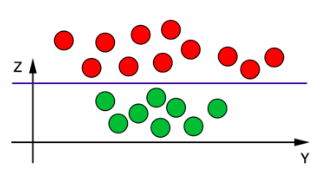
\includegraphics[width=0.9\textwidth]{SVM_NonLinear_Images/AIML_SVM_IMG10.png}
        \end{column}
\end{columns}

\end{frame}


{\1   
\begin{frame}
\title{Thanks!!}
	\subtitle{Questions?}
	\titlepage
\end{frame}
}


\end{document}
